\documentclass{tufte-handout}

\usepackage{ntheorem}
\usepackage{graphicx}
\usepackage{amsmath}
\usepackage{amssymb}
\usepackage{hyperref}
\usepackage{epigraph}
\usepackage{booktabs}
\theoremstyle{break}
% \usepackage[
% bibencoding=utf8,% .bib file encoding
% maxbibnames=3, % otherwise et al
% minbibnames=1, % otherwise et al
% backend=biber,%
% sortlocale=en_US,%
% style=apa,% or authoryear
% % apabackref=false, % backreferences
% natbib=true,% for citet/citep, but this is for backward compatibility
% uniquename=false,%
% url=true,%
% sortcites=false,
% doi=true,%
% eprint=true%
% ]{biblatex}
% \addbibresource{lecture_note_bib.bib}

\hypersetup{
  colorlinks,
  urlcolor = blue,
  pdfauthor={Paul Goldsmith-Pinkham}
  pdfkeywords={econometrics}
  pdftitle={Lecture Notes for Applied Empirical Methods}
  pdfpagemode=UseNone
}
\newtheorem{ruleN}{Rule}
\newtheorem{thmN}{Theorem}
\newtheorem{assN}{Assumption}
\newtheorem{defN}{Definition}
\newtheorem{exmp}{Example}
\newtheorem{cmt}{Comment}
\newtheorem{proof}{Proof}

\newcommand{\continuation}{??}
\newtheorem*{excont}{Example \continuation}
\newenvironment{continueexample}[1]
 {\renewcommand{\continuation}{\ref{#1}}\excont[continued]}
 {\endexcont}
\newcommand{\bY}{\mathbf{Y}}
\newcommand{\bX}{\mathbf{X}}
\newcommand{\bD}{\mathbf{D}}
\newcommand{\E}{\mathbb{E}}

\newcommand\independent{\protect\mathpalette{\protect\independenT}{\perp}}
\def\independenT#1#2{\mathrel{\rlap{$#1#2$}\mkern2mu{#1#2}}}
\DeclareMathOperator{\Supp}{Supp}

\usepackage{cleveref}
\crefname{appsec}{appendix}{appendices}
\crefname{appsubsec}{appendix}{appendices}
\crefname{assumption}{assumption}{assumptions}
\crefname{equation}{equation}{equations}
\crefname{exmp}{example}{examples}
\crefname{assN}{assumption}{assumptions}
\crefname{cmt}{comment}{comments}
\crefname{defN}{definition}{definitions}

\usepackage[nolist]{acronym}
\begin{acronym}
  \acro{CI}{confidence interval}%
  \acro{OLS}{ordinary least squares}%
  \acro{CLT}{central limit theorem}%
  \acro{IV}{instrumental variables}%
  \acro{ATE}{average treatment effect}%
  \acro{RCT}{randomized control trial}%
  \acro{SUTVA}{stable unit treatment value assignment}
  \acro{VAM}{value-added model}%
  \acro{LAN}{locally asymptotically normal}%
  \acro{DiD}{difference-in-differences}%
  \acro{OVB}{omitted variables bias}
  \acro{FWL}{Frisch-Waugh-Lovell}
  \acro{DAG}{directed acyclic graph}
  \acro{PO}{potential outcomes}
\end{acronym}

\def\inprobHIGH{\,{\buildrel p \over \rightarrow}\,} 
\def\inprob{\,{\inprobHIGH}\,} 
\def\indistHIGH{\,{\buildrel d \over \rightarrow}\,} 
\def\indist{\,{\indistHIGH}\,}

\usepackage[many]{tcolorbox} 
\definecolor{main}{HTML}{5989cf}    % setting main color to be used
\definecolor{sub}{HTML}{cde4ff}     % setting sub color to be used
\definecolor{sub2}{HTML}{fde9ce}     % setting sub color to be used

\tcbset{
    sharp corners,
    colback = white,
    before skip = 0.2cm,    % add extra space before the box
    after skip = 0.5cm      % add extra space after the box
}                           % setting global options for tcolorbox

\newtcolorbox{boxD}{
    colback = sub, 
    colframe = main, 
    boxrule = 0pt, 
    toprule = 3pt, % top rule weight
    bottomrule = 3pt % bottom rule weight
}


\newtcolorbox{boxF}{
    colback = sub2,
    enhanced,
    boxrule = 1.5pt, 
    colframe = white, % making the base for dash line
    borderline = {1.5pt}{0pt}{main, dashed} % add "dashed" for dashed line
}

\usepackage{colortbl}


\usepackage{tikz}
\usepackage{verbatim}
\usetikzlibrary{positioning}
\usetikzlibrary{snakes}
\usetikzlibrary{calc}
\usetikzlibrary{arrows}
\usetikzlibrary{decorations.markings}
\usetikzlibrary{shapes.misc}
\usetikzlibrary{matrix,shapes,arrows,fit,tikzmark}

\title{Lecture 2 -Research Designs and Model vs. Design-Based Causal Inference}
\author{Paul Goldsmith-Pinkham}
\date{\today}


\begin{document}

\maketitle
There are three goals for this set of notes:
\begin{enumerate}
  \item Discuss the value of randomized interventions, and more generally identifying settings where interventions are ``as-if'' randomly assigned. In doing so, we'll touch on the historical and (somewhat) current views on this.
  \item Define a ``research design.''
  \item Give an introduction to design-based vs. model-based identification and causal inference.
\end{enumerate}

\section{Randomization}
Randomization is a powerful tool. Being able to truly randomize an intervention allows the researcher to assume (by definition) that the potential outcomes for units are independent, satisfying the first assumption in strong ignorability.


\begin{figure}
  \begin{center}
    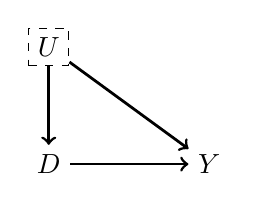
\begin{tikzpicture}
      % nodes %
      % \node[text centered] (z) {$Z$};
      \node[text centered] (t) {$D$};
      \node[right=1.5 of t, text centered] (y) {$Y$};
      \node[draw, rectangle, dashed, above = 1 of t, text centered] (u) {$U$};

      % edges %
      % \draw[->, line width= 1] (z) --  (t);
      \draw [->, line width= 1] (t) -- (y);
      % \draw[->,red, line width= 1,dashed] (u) --node {X} (z);
      \draw[->,line width= 1] (u) --(t);
      \draw[->,line width= 1] (u) -- (y);
      %\draw[->, red, line width=1,dashed] (z) to  [out=270,in=270, looseness=0.5] node{X} (y);
    \end{tikzpicture}
    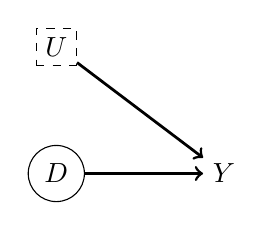
\begin{tikzpicture}
      % nodes %
      % \node[text centered] (z) {$Z$};
      \node[draw, circle, text centered] (t) {$D$};
      \node[right=1.5 of t, text centered] (y) {$Y$};
      \node[draw, rectangle, dashed, above = 1 of t, text centered] (u) {$U$};

      % edges %
      % \draw[->, line width= 1] (z) --  (t);
      \draw [->, line width= 1] (t) -- (y);
      % \draw[->,red, line width= 1,dashed] (u) --node {X} (z);
      %\draw[->,line width= 1] (u) --(t);
      \draw[->,line width= 1] (u) -- (y);
      %\draw[->, red, line width=1,dashed] (z) to  [out=270,in=270, looseness=0.5] node{X} (y);
    \end{tikzpicture}
  \end{center}
  \caption{$D$'s effect on $Y$ is confounded by $U$, but a randomized intervention of $D$ breaks any back-door connection}
\end{figure}


In a DAG, randomization ensures that any backdoor path to $D$ is broken, since the randomization was the only cause of the intervention. This allows identification of the total effect on $Y$.\footnote{Randomization does not necessarily identify the direct effect of $D$ on $Y$. For example, if $D$ affects multiple outcomes, $X$ and $Y$, and then $X$ affects $Y$ as well, it's possible that agents may reoptimize their $X$, thereby offsetting (or increasing) the direct effect of $D$ on $Y$.}

If the use of randomization is so powerful, why don't we always use it? There are a few reasons:

\begin{enumerate}
  \item People may not want to be randomized into different treatments. They value their choices, and it may be impractical to randomize their decisions even if there is a clear benefit to doing so. A firm, for example, may not want to randomize their policies (although they want to in some cases, as in settings with A/B testing).
  \item It may be unethical to randomize. For example, if there is a clear benefit to a treatment, it may be unethical to withhold that treatment from individuals by placing them in the control.\footnote{The concept of ``equipoise'' is often used to describe the ethical considerations of randomization in the medical literature \citep{freedman1987equipoise}: ``if there is
          genuine uncertainty within the expert medical
          community — not necessarily on the part of the
          individual investigator — about the preferred treatment.''}
  \item It may be impossible to randomize. For example, if we are interested in the effect of a policy change, it may be impossible to randomize the policy change across different regions or states.
\end{enumerate}


\subsection{The credibility revolution -- then and now}
While randomization is often viewed as the gold standard for policy evaluation, this was not always the case. In fact, the use of randomized experiments in economics is relatively new. Indeed, while there was the occasional agricultural economics application that had true randomization, most econometric modeling estimating causal effects and structural parameters was based on arguments about models and controls. This led to substantial skepticism in the broader community by the end of the 1970s. This can be seen in discussion about econometric estimates in \citet{leamer1983let}, ``Let's take the con out of econometrics'':\footnote{This \citet{leamer1983let} article is really worth reading in full.}

\begin{quote}
  After three decades of churning out estimates, the econometrics club finds itself under critical scrutiny and faces incredulity as never before. Fischer Black writes of ``The Trouble with Econometric Models.'' David Hendry queries "Econometrics: Alchemy or Science?" John W. Pratt and Robert Schlaifer question our understanding of "The Nature and Discovery of Structure." And Christopher Sims suggests blending "Macroeconomics and Reality.
\end{quote}

Quite explicitly, \citet{black1982trouble} says: ``The trouble with econometric models is that they present correlations disguised as causal relations. The more obvious confusions between correlation and causation can often be avoided, but there are many subtle ways to confuse the two; in particular, the language of econometrics encourages this confusion.''

The state of applied research is summarized (in a somewhat extreme way) by Leamer as:

\begin{quote}
  Econometricians would like to project the image of agricultural experimenters who divide a farm into a set of smaller plots of land and who select randomly the level of fertilizer to be used on each plot. If some plots are assigned a certain amount of fertilizer while others are assigned none, then the difference between the mean yield of the fertilized plots and the mean yield of the unfertilized plots is a measure of the effect of fertilizer on agricultural yields. The econometrician's humble job is only to determine if that difference is large enough to suggest a real effect of fertilizer, or is so small that it is more likely due to random variation.

  This image of the applied econometrician's art is grossly misleading. I would like to suggest a more accurate one. \textbf{The applied econometrician is like a farmer who notices that the yield is somewhat higher under trees where birds roost, and he uses this as evidence that bird droppings increase yields.} However, when he presents this finding at the annual meeting of the American Ecological Association, another farmer in the audience objects that he used the same data but came up with the conclusion that moderate amounts of shade increase yields. A bright chap in the back of the room then observes that these two hypotheses are indistinguishable, given the available data. He mentions the phrase ``identification problem,'' which, though no one knows quite what he means, is said with such authority that it is totally convincing.\footnote{It continues: ``The meeting reconvenes in the halls and in the bars, with heated discussion whether this is the kind of work that merits promotion from Associate to Full Farmer; the Luminists strongly opposed to promotion and the Aviophiles equally strong in favor.''}
\end{quote}

Finally, Leamer argues that the reason randomization is so helpful is that it removes the need to arbitrarily try many specifications to check for robustness to other confounding causes:

\begin{quote}
  The truly sharp distinction between inference from experimental and inference from nonexperimental data is that experimental inference sensibly admits a conventional horizon in a critical dimension, namely the choice of explanatory variables. If fertilizer is randomly assigned to plots of land, it is conventional to restrict attention to the relationship between yield and fertilizer, and to proceed as if the model were perfectly specified... In contrast, it would be foolhardy to adopt such a limited horizon with nonexperimental data. \textbf{But if you decide to include light level in your horizon, then why not rainfall; and if rainfall, then why not temperature; and if temperature, then why not soil depth, and if soil depth, then why not the soil grade; ad infinitum.} Though this list is never ending, it can be made so long that a nonexperimental researcher can feel as comfortable as an experimental researcher that the risk of having his findings upset by an extension of the horizon is very low. The exact point where the list is terminated must be whimsical, but the inferences can be expected not to be sensitive to the termination point if the horizon is wide enough.
\end{quote}

If we fast-forward 25 years, \citet{angrist2010credibility} have now declared victory: ``The credibility revolution in empirical economics: How better research design is taking the con out of econometrics'':
\begin{quote}
  Empirical microeconomics has experienced a credibility revolution, with a consequent increase in policy relevance and scientific impact. Sensitivity analysis played a role in this, but as we see it, the primary engine driving improvement has been a focus on the quality of empirical research designs...
  The advantages of a good research design are perhaps most easily apparent in research using random assignment, which not coincidentally includes some of the most influential microeconometric studies to appear in recent years.
\end{quote}

As evidenced by both the title and the quote above, \textbf{research design} is declared the victor. But what is a research design? And why is randomization its champion?

\begin{boxD}
  \begin{exmp}
    Some famous examples of programs that used randomization (including those that they cite) include:
    \begin{itemize}
      \item PROGRESA, a conditional cash transfer program in Mexico (see \citet{parker2017conditional} for a review)
      \item Moving to Opportunity (MTO), a program that randomly selected low income families to receive housing vouchers (see \citet{katz2001moving} for a discussion on the program)
      \item National Supported Work (NSW) demonstration, a federal job training program that was randomized amongst applicants (\citet{lalonde1986evaluating} is the canonical paper whose work with this program is what sparked the ``credibility revolution'' -- we will discuss this next class)
      \item Oregon health insruance experiment, where the state of Oregon randomized its Medicaid program for low-income, uninsured adults. See \citet{baicker2013oregon} for a discussion.
      \item Tennessee STAR class size experiment, which randomized students into classrooms of different sizes. See \citet{krueger1999experimental} for a discussion.
      \item H\&R Block FAFSA was field experiment where individuals recieving tax preperation at H\&R Block  were randomized into a procedure to get help on the Free Application for Federal Student Aid (FAFSA).  See \citet{bettinger2012role} for a discussion.
    \end{itemize}
  \end{exmp}
\end{boxD}

\section{What is a research design?}
A goal of this class, and your empirical research going forward, is to have a precise research design for your empirical analyses. This is a term that is used frequently, but not always clearly defined. In fact, in the \citet{angrist2010credibility} paper, the term is never defined explicitly, despite being mentioned 69 times. I have seen it defined explicitly only a few times, and rarely in economics.\footnote{One very nice text in political science that does define it  is \citet{blair2023research}.  They define a research design as ``a procedure for generating answers to questions.''}

I will provide you a definition, with the understanding that this is not the only definition, and that there are many different ways to think about research design. Much of the value in thinking about a research design is about being explicit about the assumptions that you are making, and how you are using the data to answer your question.

A research design is a statistical and/or economic statement of how to estimate a causal relationship between two variables of interest: how $X$ causes $Y$. Since we know that causal effects require the estimation of an (unobservable) counterfactual, this statement describes the assumptions necessary to impute the counterfactual. Why is this valuable?

First, it forces you to articulate \emph{what} the counterfactual is. This may seem obvious, but often you may find researchers estimating a linear equation and presenting estimates without clearly thinking about their counterfactual statement. For example, when you estimate the effect of a policy change, what is the counterfactual? Is it the state of the world where the policy never occured? Or is it one where the policy was introduced later? Or when estimating the effect of an informational event (such as the effect of monetary policy), is the counterfactual where the event never occurred? Or is it where the event occurred as previously expected?

Second, it forces you to articulate \emph{how} you are going to estimate the counterfactual, and what assumptions are necessary. This is, of course, what we will spend the rest of the semester building tools to do. But at a very high-level, a research design can be split into two types of approaches: model-based and design-based. Model-based approaches will involve assumptions about modeling the expectation (or other functional) of the counterfactual, specifically dealing with any possible confounding variables. Design-based approaches will involve assumptions about the treatment assignment mechanism, without making formal assumptions about the model of the potential outcomes.

\begin{boxF}
  \begin{cmt}
    \begin{itemize}
      \item Model-based: the estimand is
            identified using assumptions on the modeling of the potential outcomes conditional on treatment and additional variables
            (e.g. parallel trends). Examples of approaches that can fall under this category include difference-in-differences (including non-random staggerred diff-in-diff), regression discontinuity, synthetic control (and synthetic diff-in-diff), and instrumental variable approaches that use ``included'' instruments.
      \item Design-based: the estimand is identified using assumptions on the treatment variable,
            conditional on the potential outcomes and additional variables. Examples include randomized control trials, instrumental variable approaches that use ``excluded'' instruments, difference-in-difference with \emph{random} staggered timing, and propensity score matching.
    \end{itemize}
    See \href{https://twitter.com/lihua_lei_stat/status/1479700463343714306?s=20&t=pKi-XTp3e89Rn8KV8b3KEA}{Lihua Lei's very nice twitter thread} for a small history on why these terms acquired their labels.
  \end{cmt}
\end{boxF}

To give a concrete example of how these assumptions may differ, we can use the example from \citet{robins1992estimating}. Consider the question of how smoking affects peoples' ability to breath, as measured by ``forced expiratory volume in one second'' (FEV1). This is often used as a measure of lung function. Now we want to know what the effect of a person being a smoker ($D_{i}$) is on the individuals' FEV1 ($Y_{i}$).  The two approaches (model and design) highlight the different ways you might consider estimating the effect. One approach would be to think hard about ways that shift around an individuals' propensity to be a smoker in as-if random ways -- this would be a \emph{design} approach, since it is focused on the treatment assignment mechanism.  Another approach might be to compare individuals over time in places where cigarette smoking was legal earlier vs. later -- this would be a \emph{model} approach, since it is focused on the modeling of the potential outcomes by using the individuals in the state with later smoking as a control for the earlier group.\footnote{One could take the \emph{same} data and use it for both approaches. If you were willing to assume that the states chose to make the cigarettes legal late vs. early randomly, then this would be a design-based approach, since it would influence the treatment assignment mechanism.}

As it turns out, not only do these approaches matter for clarity of thought, they matter for robustness of estimation (design-based inference will be robust to model specification), weighting of estimands (model-based approaches will be more sensitive to negative weights), and the ability to generalize to other settings (model-based approaches are often more easily generalized, conditional on the model being correct). Moreover, one approach, with the same research data and causal question, may be much more statistically precise than another. We will continue to explore and describe these two approaches throughout the semester.


\section{Randomization and design-based inference}
Returning to randomization,  we can see that randomized interventions are a form of design-based causal inference. Konwledge of the treatment assignment mechanism gives a very powerful tool for thinking about the counterfactual. In fact, it is so powerful that it is the benchmark for other approaches in design-based inference. That is, a randomized intervention with knowledge of the treatment assignment mechanism is the ``gold standard.'' In future cases, we will need to make assumptions about the treatment assignment mechanism and defend them. For now, we will provide the notation and estimators for the randomized case, and next class we will discuss more general approaches.

As before, there is a finite population of $n$ individuals indexed by $i$. For each $i$, we have triplets $(Y_{i}(0), Y_{i}(1), D_{i})$,  where   $D_{i} \in \{0,1\}$  is the treatment status and $(Y_{i}(0), Y_{i}(1))$ denotes the potential outcomes. We observe $(Y_{i}, D_{i})$, and define the vector version of these as $\bY$ and $\bD$.  There are many things we could want to know abotu the relationship between $D_{i}$ and $\tau_{i} = Y_{i}(1) - Y_{i}(0)$, but for today, we will focus on $\bar{\tau} = n^{-1}\sum_{i=1}^{n}\tau_{i}.$\footnote{One could, for example, study the median treatment effect, or other features of the distribution. This is more complex, as we will see in future lectures.}

Design-based inference considers the set of potential ways that $\mathbf{D}$ could be randomized to the population. We will assume that $\mathbf{Y}_{1}$ and $\mathbf{Y}_0$ are \emph{fixed} -- it is only the random variation in $\mathbf{D}$ that creates uncertainty. Formally, let $\Omega$ denote that space of possible values that $\mathbf{D}$ can take. It is defined by the type of randomized experiment one runs.

\begin{boxD}
  \begin{exmp}
    If we do a purely randomized individualized trial, where
    each individual has a fair coin flipped on whether they are
    treatment or control, then $\Omega = \{0,1\}^{n}$. But then
    the variation in number treated and control can vary quite a
    lot for small samples!

    \centering
    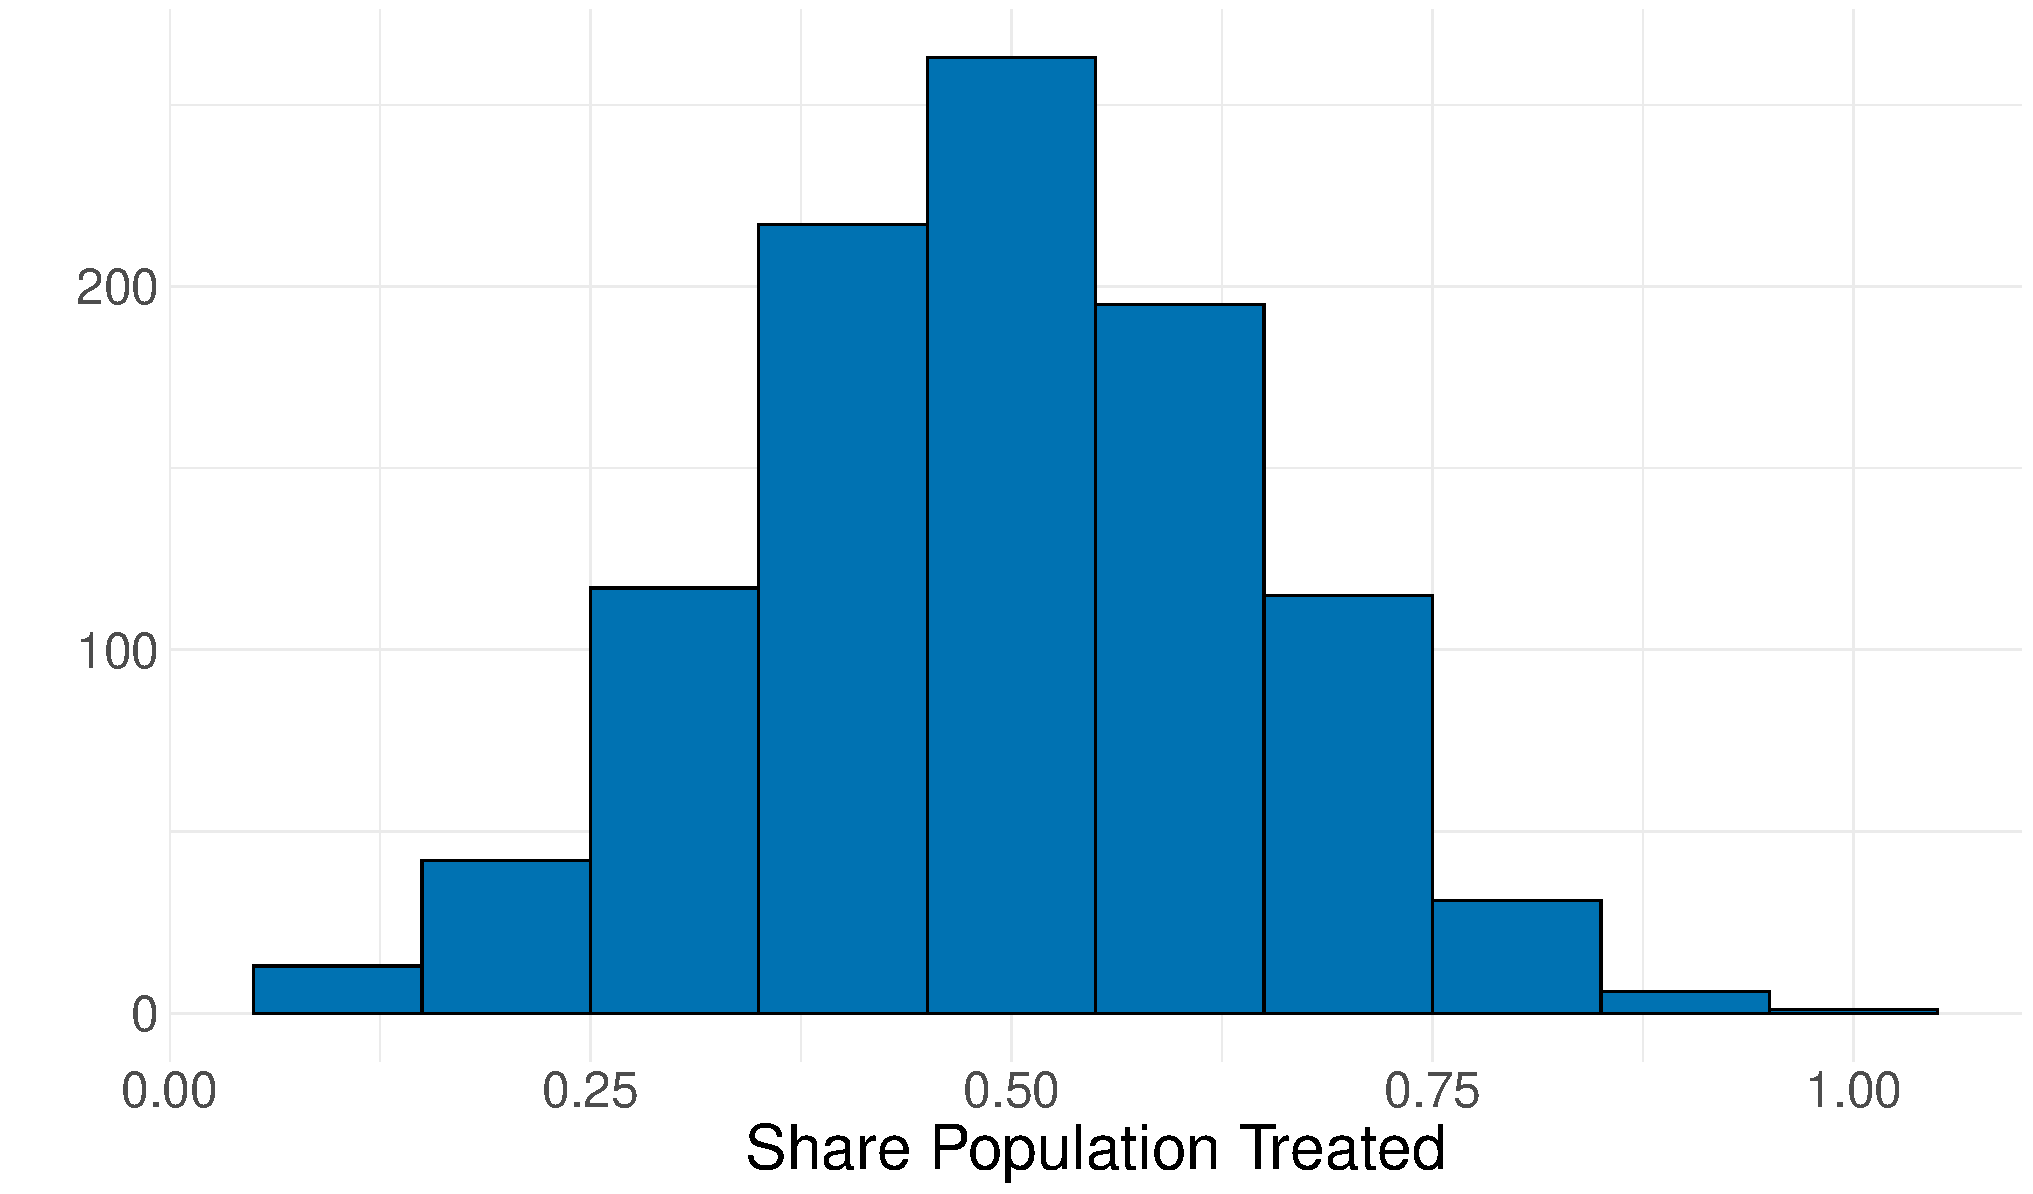
\includegraphics[width=0.5\linewidth]{../lectures/images/randomized1.pdf}

    \raggedright
    Other ways to consider randomly assigning individuals include:
    \begin{itemize}
      \item Random draws from an urn (to ensure an exact number treated)
      \item Clustering individuals on characteristics (or location)
    \end{itemize}
  \end{exmp}
\end{boxD}

Given our sample space and knowledge of the randomziation, we know the exact probability distribution over $\Omega$, and hence $\mathbf{D}$.

\begin{boxD}
  \begin{exmp}
    \label{example1_randomization}
    Consider a sample of 10 units, with 5 treated and 5 control. We know that there are only ${10 \choose 5}= 252$ potential combinations (each equally likely).  We observe one set of them in  \Cref{tab:ex_randomized1}. Note that one set of the entries (in blue) are fundamentally unobservable due to the treatment status.
  \end{exmp}
\end{boxD}
\begin{margintable}
  \begin{tabular}{crrrr}
    \toprule
    $D_{i}$ & $Y_{i}(1)$              & $Y_{i}(0)$              & $Y_{i}$ & $\tau_{i}$               \\
    \midrule
    1       & 11.9                    & \cellcolor{main!25} 6.6 & 11.9    & \cellcolor{main!25}5.3  \\
    1       & 10.0                    & \cellcolor{main!25} 8.5 & 10.0    & \cellcolor{main!25}1.5  \\
    1       & 9.7                     & \cellcolor{main!25} 9.4 & 9.7     & \cellcolor{main!25}0.3  \\
    1       & 9.5                     & \cellcolor{main!25} 7.0 & 9.5     & \cellcolor{main!25}2.5  \\
    1       & 11.4                    & \cellcolor{main!25} 7.4 & 11.4    & \cellcolor{main!25}4.0  \\
    0       & \cellcolor{main!25} 9.6 & 7.6                     & 7.6     & \cellcolor{main!25}2.0  \\
    0       & \cellcolor{main!25}9.1  & 7.1                     & 7.1     & \cellcolor{main!25}2.0  \\
    0       & \cellcolor{main!25}10.4 & 7.7                     & 7.7     & \cellcolor{main!25}2.7  \\
    0       & \cellcolor{main!25}10.4 & 8.0                     & 8.0     & \cellcolor{main!25} 2.4 \\
    0       & \cellcolor{main!25}12.4 & 7.8                     & 7.8     & \cellcolor{main!25}4.6  \\
    \bottomrule
  \end{tabular}
  \caption{Example of a randomization over $n = 10$ units. The highlighted entries are unobservable due to the fundamental problem of causal inference.}
  \label{tab:ex_randomized1}
\end{margintable}



Now, we need an estimator for $\bar{\tau} = n^{-1}\sum_{i=1}^{n}\tau_{i}$. We already know under random assignment that $E(Y_{i}| D_{i} = 1) - E(Y_{i} | D_{i} = 0)$ identifies $E(\tau_{i})$. Then, the empirical analog is quite easy (with $n_{1}$ equal to the number of treated, $n_{0}$ number control, and $n_{0} + n_{1} = n$):
\begin{align}
  \hat{\bar{\tau}}(\mathbf{D}, \mathbf{Y}) & =   \frac{\mathbf{D}'\mathbf{Y}}{\sum_{i}D_{i}} - \frac{(\mathbf{1}-\mathbf{D})'\mathbf{Y}}{\sum_{i}(1-D_{i})} \\
                                           & = n_{1}^{-1}\sum_{i} Y_{i}D_{i} -  n_{0}^{-1}\sum_{i} Y_{i}(1-D_{i})
\end{align}
Note that this expectation operator is well-defined from the objects we already know. Since only $D$ is random, and we know its marginal distribution over the sample we can show that this estimator is unbiased. This particular estimator is unbiased when the \emph{design}, or the randomization across $\Omega$, is special: it has complete random assignment across of the units across the treatment. We assume that $n_{1}/n$ units are randomly assigned (in our example in \Cref{tab:ex_randomized1}, $5/10$.).\footnote{If the probabiltiies vary across the sample space (due to covariates, say, or a more unusual sampling scheme), we need to add weights. This is known as Horovitz-Thompson weighting, and we will return to this.}

Under this design,the probability of a unit receiving treatment given a draw $\bD$ is $\pi = n_{1}/n$. Note that this implies that there are always $n_{1}$ units treated, and we are randomly allocating the treatments within the $n$ units. Then, note that $E(\pi_{1}^{-1}D_{i}) = 1$.\footnote{Recall that $E(D_{i}) = Pr(D_{i} = 1) =  n^{-1}n_{1}.$} With this,

\begin{align*}
  E(\hat{\bar{\tau}}(\mathbf{D}, \mathbf{Y})) & = E\left(\frac{\mathbf{D}'\mathbf{Y}}{\sum_{i}D_{i}} - \frac{(\mathbf{1}-\mathbf{D})'\mathbf{Y}}{\sum_{i}(1-D_{i})}\right) \\
  & =n^{-1}E\left(\sum_{i}\pi_{1}^{-1}Y_{i}D_{i} - \sum_{i}(1-\pi_{1})^{-1}Y_{i}(1-D_{i})\right)                               \\
& =n^{-1}E\left(\sum_{i}\pi_{1}^{-1}Y_{i}(1)D_{i} - \sum_{i}(1-\pi_{1})^{-1}Y_{i}(0)(1-D_{i})\right)                         \\
& =n^{-1}\sum_{i}Y_{i}(1)E\left(\pi_{1}^{-1}D_{i}\right) - n^{-1}\sum_{i}Y_{i}(0)E\left((1-\pi_{1})^{-1}(1-D_{i})\right)     \\
    & =n^{-1}\sum_{i}Y_{i}(1) - Y_{i}(0) = n^{-1}\sum_{i}\tau_{i}.
\end{align*}
Hence, this estimator is unbiased for the ATE.

We can also study the variance properties of the estimator. Thanks to \citet{neyman1990}, we know that the variance of $\hat{\bar{\tau}}$ is given by:
\begin{equation}
  \sigma^{2}_{\hat{\bar{\tau}}} = \frac{1}{n-1}\left(\frac{n_{1}\sigma^{2}_{0}}{n_{0}} + \frac{n_{0} \sigma^{2}_{1}}{n_{1}} + 2\sigma_{0,1}\right)
\end{equation}
where $\sigma^{2}_{0}, \sigma^{2}_{1}, \sigma_{0,1}$ are the variance of the potential control, treatment, and the covariance between the two. Note that these variances are of the potential outcomes. Some nice intuition can come from looking at this. First, we see that the variance of the estimator increases when either the treated or control variance increases. This makes sense -- it is harder to distinguish treatment and control when there is a large dispersion for either group. Second, the overall variance is increases (holding fixed the specific variances) as you increase the share of treated units. This makes sense because you have less information about the control for the treatment. Finally, the covariance of the potential outcomes matters for the overall variance -- if the units have negative covariance, that will help in estimating the treatment effect because a large shock to the control potential outcome will be offset by a large shock in the other direction for the treatment.

Since we do not know $\sigma_{0,1}$, we need to bound this estimand with a conservative estimator:
\begin{equation}
  \hat{\sigma}^{2}_{\hat{\bar{\tau}}} = \frac{n}{n-1}\left(\frac{\hat{\sigma}^{2}_{0}}{n_{0}} + \frac{ \hat{\sigma}^{2}_{1}}{n_{1}}\right).
\end{equation}
This estimator is knowable from the data, if the treatment is randomly assigned. 

\begin{boxD}
  \begin{continueexample}{example1_randomization}
    \label{example2_randomization}
    We can now construct our estimator and the variance of this estimator:
    \begin{equation*}
      \hat{\bar{\tau}} = 5^{-1}\sum_{i}Y_{i}D_{i} - 5^{-1}\sum_{i}Y_{i}(1-D_{i}) = 2.86
    \end{equation*}
    and
    \begin{align*}
      \hat{\sigma}^{2}_{0} &= 5^{-1}\sum_{i}(Y_{i}-\hat{\overline{Y}}_{0})^{2}(1-D_{i}) = 0.932\\
       \hat{\sigma}^{2}_{1} &= 5^{-1}\sum_{i}(Y_{i}-\hat{\overline{Y}}_{1})D_{i} = 0.0904\\
      \hat{\sigma}^{2}_{\hat{\tau}} &= \frac{10}{9}\left(\frac{0.932}{5} + \frac{0.0904}{5}\right) =  0.2
    \end{align*}
    Hence, our standard error is $\sqrt{0.2} = 0.45$.
  \end{continueexample}
\end{boxD}

\begin{boxF}
  \begin{cmt}
    It is interesting to note that this variance estimator is nearly identical to the case with the standard robust estimator from a more traditional linear equation:
    \begin{equation*}
      Y_{i} = \alpha + \beta D_{i} + \epsilon_{i}.
    \end{equation*}
    See Equation 2 from \citet{imbens2016robust} to compare. 
  \end{cmt}
\end{boxF}

\subsection{Thinking about inference}
We could use this variance estimator to thinking about constructing \emph{confidence intervals} now. Often, this is done by inverting a hypothesis test. For example, we could test the null hypothesis that $E(\tau_{i}) = 0$ -- the average treatment effect in the sample is zero. We will revisit this in further detail in our linear regression classes, and you have likely seen quite a bit of this in your previous classes. Thinking about testing in the design-based setting will be no different -- the only change is that the uncertainty is driven by the random assignment of the treatment, rather than uncertainty in the outcome (e.g. usually the errors in the model). It is not always easy to figure out \emph{what} the variance of an estimator is that has a non-standard design. We will discuss simple cases where probabilities are done in a straightforward way, but often experiments are run in ways that create unusual dependence across units.\footnote{See \citet{imbens2015causal} for a general discusion and \citet{chang2023design} for a discussion on complex experiements.}

One very powerful tool that can avoid estimation of standard errors is to use randomization inference instead. One example where we can use this is in testing the strong null hypothesis that $\tau_{i} = 0$ for \emph{all} $i$. That is, the treatment has zero effect. This is a very strong null hypothesis -- it is stronger than the null hypothesis that $\bar{\tau} = 0$. 

\begin{margintable}
  \begin{tabular}{cccc}
 \toprule
 $D_{i}$ & $Y_{i}(1)$ & $Y_{i}(0)$ & $Y_{i}$\\
 \midrule
 1 &  11.9 & 11.9  & 11.9\\
 1 &  10   & 10  & 10\\
 1 &  9.7  & 9.7  & 9.7\\
 1 &  9.5  & 9.5 & 9.5 \\
 1 &  11.4 & 11.4  & 11.4\\
 0 & 7.6  &  7.6 & 7.6\\
 0 &  7.1  & 7.1  & 7.1\\
 0 &  7.7 &  7.7  & 7.7\\
 0 & 8  &  8 & 8  \\
 0 & 7.8  & 7.8 & 7.8\\
 \bottomrule
 \end{tabular}
 \caption{Imputed values under the null hypothesis of $\tau_{i} = 0$ for all $i$.}
\end{margintable}
 Given our data and under the null of $\tau_{i} = 0$, we can calculate the full distribution of potential observed statistics we would see, as we vary $D$. We do so by imputing our missing values under the null hypothesis, and calculating the estimator if we randomly permuted the treatment labels. Since we are asserting the known missing values, we can reconstruct the full distribution in \Cref{fig:randomized2}. We can then calculate the probability of seeing a value as extreme as our observed value. This is known as a \emph{p-value}. If this probability is small, we reject the null hypothesis that $\tau_{i} = 0$ for all $i$.


\begin{figure}       
      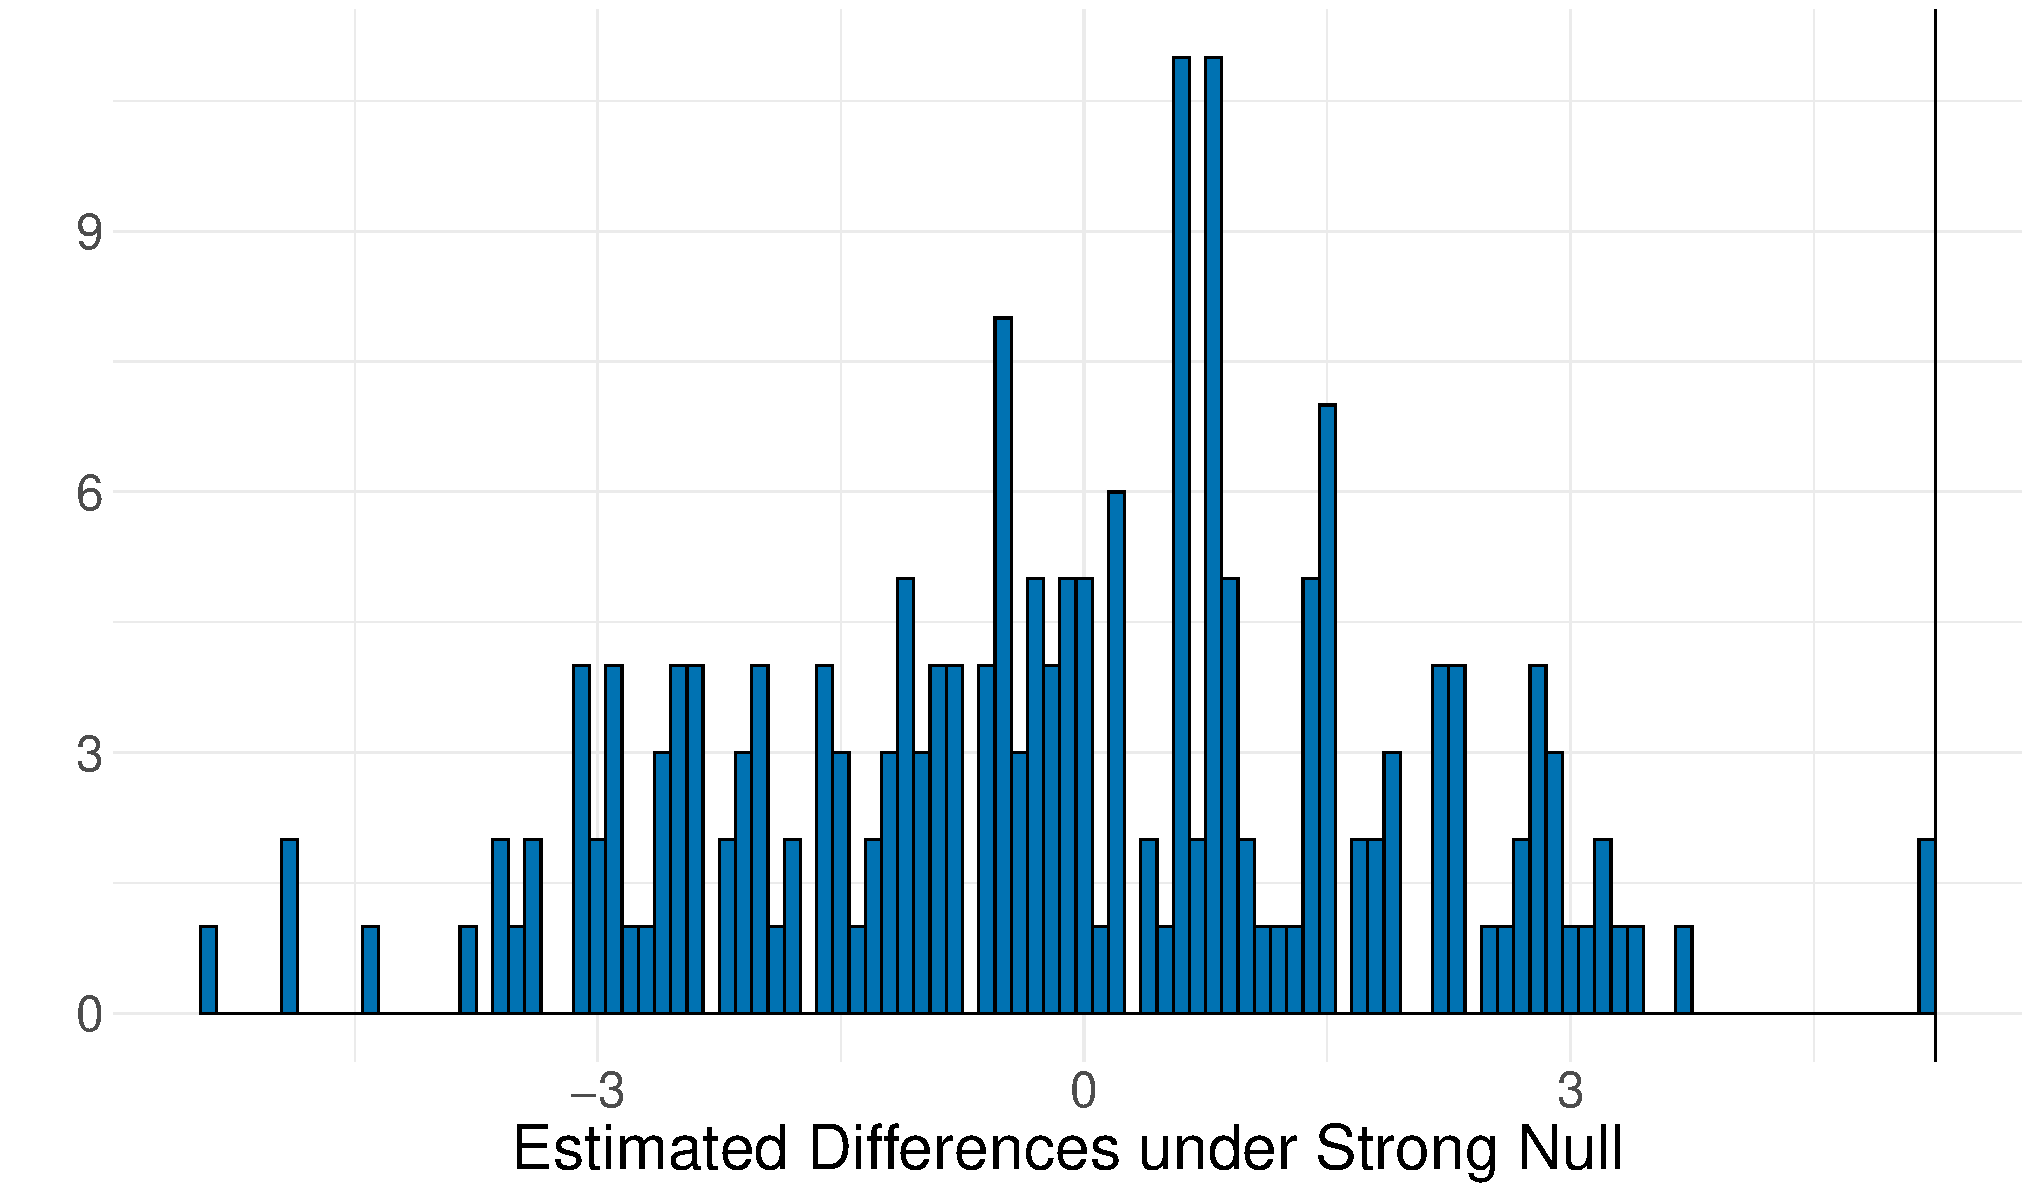
\includegraphics[width=0.9\linewidth]{../lectures/images/randomized2.pdf}
      \caption{Distribution of $\hat{\bar{\tau}}$ under the null hypothesis of $\tau_{i} = 0$ for all $i$ under all permutations. Vertical line denotes the observed estimate in the data.}
      \label{fig:randomized2}
\end{figure}

\begin{boxF}
  \begin{cmt}
    We have only discussed a very simple estimator which assumes complete randomization. The generalized estimator that allows for more complex randomization schemes is known as the Horvitz-Thompson estimator from Horvitz-Thompson (1952) (see Aronow and Middleton (2013) for a useful discussion):
    \begin{equation}
            \hat{\bar{\tau}}_{HT} = n^{-1}\left[\sum_{i}\frac{1}{\pi_{1i}}Y_{i}D_{i} - \frac{1}{\pi_{0i}}Y_{i}(1-D_{i})\right],
          \end{equation}
          where $\pi_{i1} = Pr(D_{i} = 1)$, and $\pi_{0i} = Pr(D_{i} = 0)$. This estimator is unbiased even in settings where we don't have equal weighting across the sampling space. This is reweighting using the propensity score! We will discuss this next class.
  \end{cmt}
\end{boxF}

\section{Credibility revolution and internal vs. external validty}

The focus on randomization and credible design has had an extremely powerful impact of the believability of estimates. However, there was (and sometimes is) a view that the emphasis in these approaches focuses too much on solving problems of \emph{internal validity} (i.e. the ability to identify the causal effect \emph{in the sample}) and not enough on \emph{external validity} (i.e. the ability to generalize to other settings). 

This debate around internal vs. external validity erupted at the end of the 2000s, especially focused in development economics. Papers in this space include:
    \begin{itemize}
    \item ``Instruments, Randomization, and Learning about Development'' Deaton (2010)
    \item ``Comparing IV with structural models: What simple IV can and cannot identify'', Heckman and Urzua (2009)
    \item ``Better LATE Than Nothing: Some Comments on Deaton (2009) and Heckman and Urzua (2009)'' Imbens (2010)
    \item ``Building Bridges between Structural and Program Evaluation Approaches to Evaluating Policy'' Heckman (2010)
    \end{itemize}
Much of this is tied to instrumental variables, which we'll revisit later. To give you a flavor of the issue as flagged in development, here is Angus Deaton in 2010 \citep{deaton2010instruments} describing issues with randomized experiments in development:

\begin{quote}
  Under ideal circumstances, randomized eval
 uations of projects are useful for obtaining
 a convincing estimate of the average effect
 of a program or project. The price for this
 success is a focus that is too narrow and too
 local to tell us "what works" in development,
 to design policy, or to advance scientific knowledge about development processes. Project evaluations, whether using random ized controlled trials or nonexperimental
 methods, are unlikely to disclose the secrets
 of development nor, unless they are guided
 by theory that is itself open to revision, are
 they likely to be the basis for a cumulative
 research program that might lead to a better understanding of development.
\end{quote}

As another example, here is a table from \citet{heckman2010building} that compares the assumptions needed for potential outcomes vs. structural work (a dichotomy which I think is somewhat vacuous), and emphasizing the external validity problem in potential outcomes work:\footnote{There are a number of statements in this table that are not correct regarding potential outcomes. For example, the statement that social interactions is assumed away is not correct. See Lecture 4 for more discussion.}
\begin{figure*}
  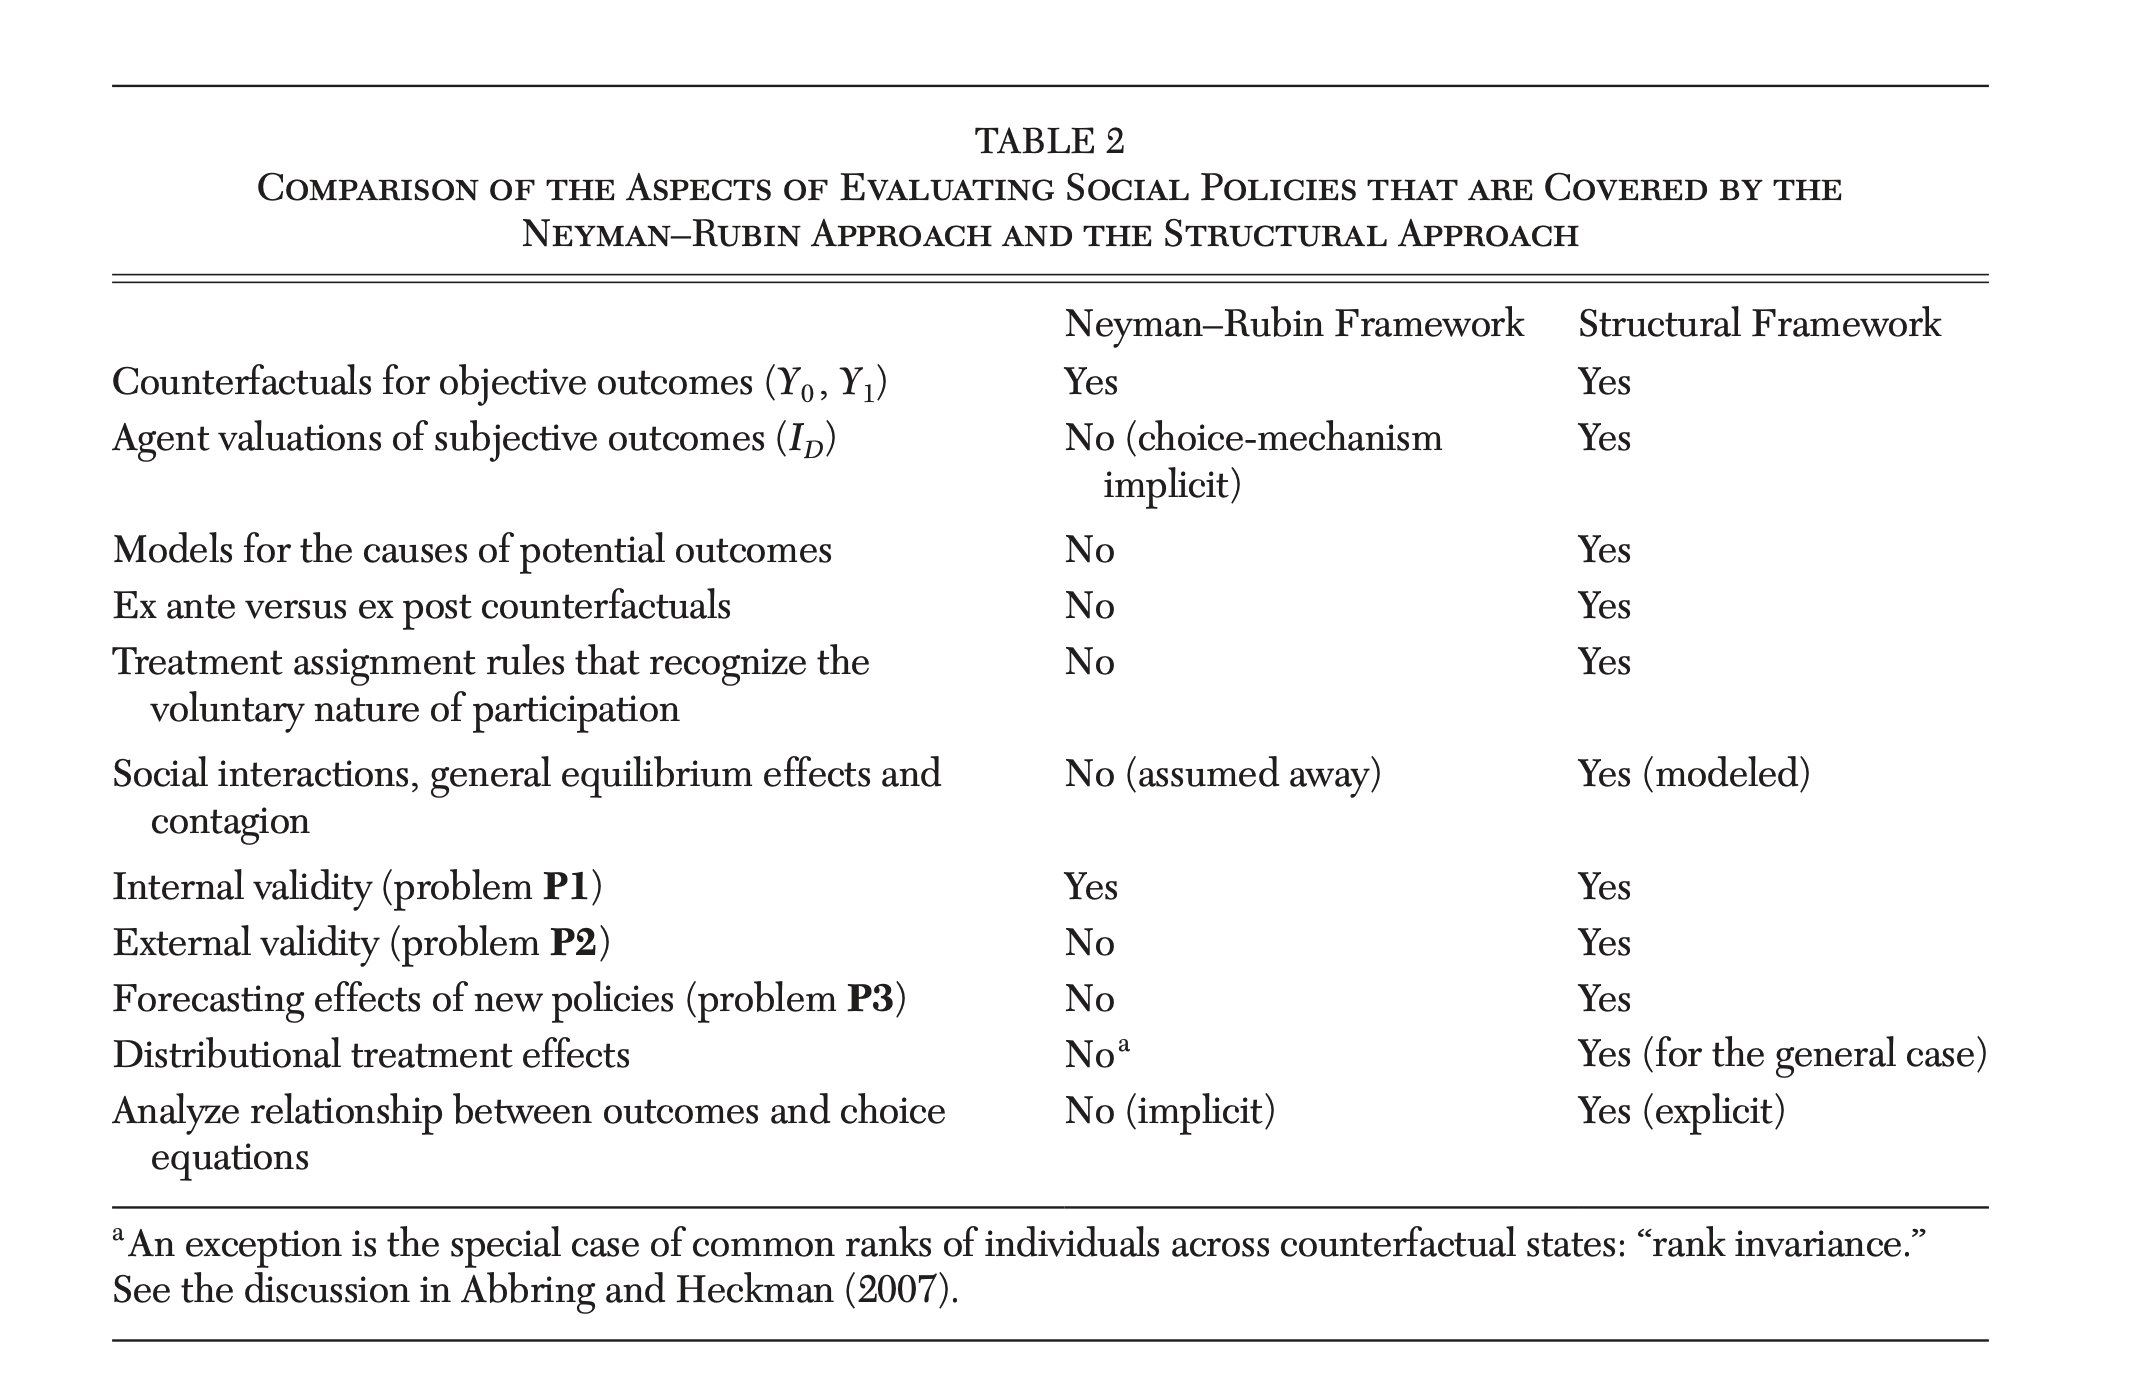
\includegraphics[width=0.8\linewidth]{../lectures/images/heckman1.jpeg}
\end{figure*}

Many of the complaints by the anti-randomistas devolve into three types: first, the analyses are done incorrectly (e.g. bad IVs). I think full-throated defenders of experiments would agree that badly done research should be rejected regardless. More importantly, the transparency of the research design should make this easier. Second, that research does not generalize to other populations. For example, Progressa is a big success, but knowing that conditional  cash transfers work in this one setting may not necessarily inform our ability to roll it out in places that are very different. Third, that there is a rhetorical overreliance on RCTs as the gold standard, and that  post-hoc analyses (without a pre-analysis plan) defeat the underlying value of an RCT anyway.\footnote{It is unclear why an experiment is worse than a non-experiment in this regard, but this is a concern Deaton flags.} More generally, there is a concern that focusing on clever RCTs and IVs causes an overfocus on irrelevant or unimportant questions. A briefcase full of results that are not economically useful.\footnote{This is still a complaint one can hear today!}

It is useful to consider these concerns in the context of the discussion at the beginning of this lecture. Much of this concern about how to do empirical work does not provide much of a counterfactual. Historical evidence suggests that empirical work was simply not credible prior to this move. Additionally, it seems like the concerns about empirics being too separated from models are overstated. Perhaps in part in response to these critiques, many empirical papers with causal parameters are  tightly linked to theretical work. For those that are not, the results eventually  inform many theoretical papers. A push to open data has actually made it easier for researchers to follow-up and study these issues. 

The key way in which ``better research design is taking the con out of econometrics'' is by making the assumptions in empirical work \emph{explicit}. This can be using a randomized intervention, or some other design-based approach, or it can be done using a model-based approach. Then, researchers can evaluate clearly the credibility of the assumptions, and the robustness of the results to these assumptions. \emph{The inclusion of an economic model does not grant an empirical researcher to omit a research design from their empirics.} Many researchers may propose a model, and then demonstrate that their model is consistent with observational data. This is not a research design, which requires an additional argument for how the empirical approach can be used to identify the causal estimand of interest.

\bibliography{lecture_note_bib.bib}
\bibliographystyle{plainnat}


\end{document}